\documentclass{jsarticle}

\usepackage{amsmath}
\usepackage{amssymb}
\usepackage{booktabs}
\usepackage{float}
\usepackage{graphicx}
\usepackage{listings}
\usepackage{url}

\lstset{
  basicstyle={\ttfamily},
  identifierstyle={\small},
  commentstyle={\smallitshape},
  keywordstyle={\small\bfseries},
  ndkeywordstyle={\small},
  stringstyle={\small\ttfamily},
  frame={tb},
  breaklines=true,
  columns=[l]{fullflexible},
  numbers=left,
  xrightmargin=0zw,
  xleftmargin=3zw,
  numberstyle={\scriptsize},
  stepnumber=1,
  numbersep=1zw,
  lineskip=-0.5ex
}

\title{情報領域演習第二 L演習(クラス3) レポート}
\author{学籍番号: 1810678 \\
        名前: 山田朔也}

\begin{document}
    \maketitle
    \begin{description}
        \item[問1.]
        \begin{description}
            \item[(a)]
            作成した状態は以下の図\ref{fig1}のようになった。また、状態遷移図がこのようになる理由は問1の(b)にて説明する
            \begin{figure}[H]
                \centering
                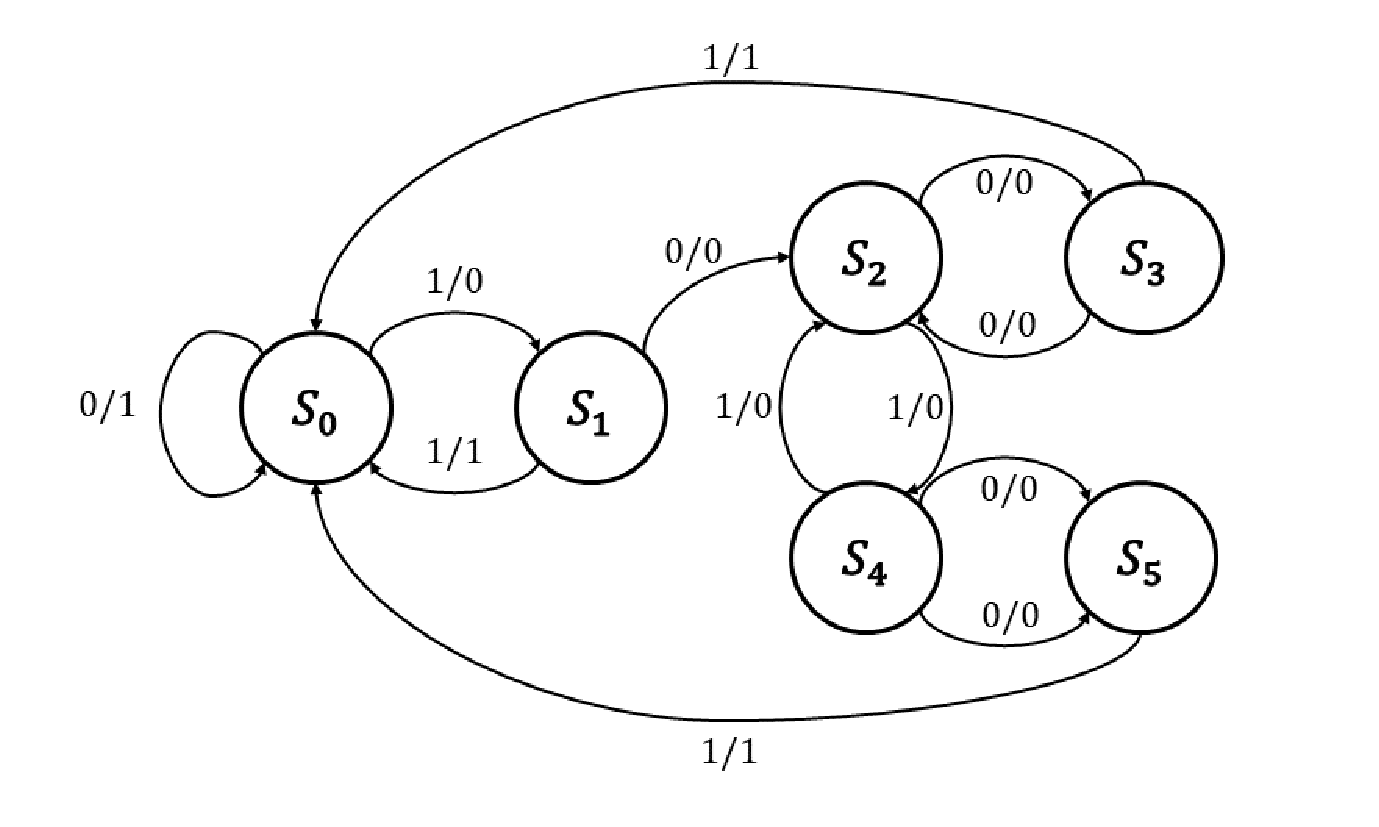
\includegraphics[width = 10cm]{fig_1.eps}
                \caption{最上位ビットから読み取った時の状態遷移図}
                \label{fig1}
            \end{figure}

            \item[(b)]
            (a)で作成した状態遷移図の状態遷移表は以下の表\ref{tab1}のようになる。
            \begin{table}[H]
                \centering
                \caption{状態遷移図\ref{fig1}の状態遷移表}
                \label{tab1}
                \begin{tabular}{|c|c|c|} \hline
                    & 0 & 1 \\ \hline
                    $S_0$ & $S_0 \,,\, 1$ & $S_1 \,,\, 0$ \\ \hline
                    $S_1$ & $S_2 \,,\, 0$ & $S_0 \,,\, 1$ \\ \hline
                    $S_2$ & $S_3 \,,\, 0$ & $S_4 \,,\, 0$ \\ \hline
                    $S_3$ & $S_2 \,,\, 0$ & $S_0 \,,\, 1$ \\ \hline
                    $S_4$ & $S_5 \,,\, 0$ & $S_2 \,,\, 0$ \\ \hline
                    $S_5$ & $S_4 \,,\, 0$ & $S_0 \,,\, 1$ \\ \hline
                \end{tabular}
            \end{table}
            ここからこの状態遷移表を講義で習ったように、等価な状態でグループ分けをしてしていくと以下の表\ref{tab2}のようになった。
            \begin{table}[H]
                \centering
                \caption{グループ分けの遷移}
                \label{tab2}
                \begin{tabular}{|c|c|c|c|} \hline
                    & 現状態 & 0 & 1 \\ \hline
                    $B_0^1$ & $S_0$ & $B_0^1$ & $B_1^1$ \\ \hline
                    $B_1^1$ & $S_1$ & $B_2^1$ & $B_0^1$ \\ \cline{2-4}
                     & $S_3$ & $B_2^1$ & $B_0^1$ \\ \cline{2-4}
                     & $S_5$ & $B_2^1$ & $B_0^1$ \\ \hline
                    $B_2^1$ & $S_2$ & $B_1^1$ & $B_2^1$ \\ \cline{2-4}
                     & $S_4$ & $B_1^1$ & $B_2^1$ \\ \hline
                \end{tabular}
            \end{table}
            これより、簡単化ができる。そして、簡単化後の状態遷移表と、その符号化を行った状態遷移表は以下の表\ref{tab3}ようになる。
            \begin{table}[H]
                \centering
                \caption{各処理後の状態遷移表}
                \label{tab3}
                \begin{minipage}{0.4\columnwidth}
                    \centering
                    \caption{簡単化後の状態遷移表}
                    \begin{tabular}{|c|c|c|} \hline
                        & 0 & 1 \\ \hline
                        $S_0^*$ & $S_0^* \,,\, 1$ & $S_1^* \,,\, 0$ \\ \hline
                        $S_1^*$ & $S_2^* \,,\, 0$ & $S_0^* \,,\, 1$ \\ \hline
                        $S_2^*$ & $S_1^* \,,\, 0$ & $S_2^* \,,\, 0$ \\ \hline
                    \end{tabular}
                \end{minipage}
                \begin{minipage}{0.4\columnwidth}
                    \centering
                    \caption{符号化後の状態遷移表}
                    \begin{tabular}{|c|c|c|} \hline
                        & 0 & 1 \\ \hline
                        00 & $00 \,,\, 1$ & $01 \,,\, 0$ \\ \hline
                        01 & $10 \,,\, 0$ & $00 \,,\, 1$ \\ \hline
                        10 & $01 \,,\, 0$ & $10 \,,\, 0$ \\ \hline
                    \end{tabular}
                \end{minipage}
            \end{table}
            ここから論理式を求めていく。まず、符号化した状態の0,1の列において下位ビットを$s_0$,上位ビットを$s_1$とする。
            また、入力は$x$,出力を$f$とすると、$s_0 \,,\, s_1 \,,\, f$のカルノー図は以下のようになる。
            \begin{table}
                \centering
                \caption{様々なカルノー図}
                \label{tab4}
                \begin{minipage}
                    
                \end{minipage}
            \end{table}

      \end{description}
  \end{description}
\end{document}
